\chapter{Introduction}
\label{ch:introduction}

\dictum[Kir Bulychev,\\Alice on Alive Planet ]{%

\begin{otherlanguage}{russian}
Есть такое наблюдение: если насморк не лечить, то он пройдет через неделю, а если лечить, то через семь дней.
\end{otherlanguage}

There's a following observation: if you don't treat the cold, it will pass in  week, but if you do, then it will pass in seven days.

}%
\vskip 1em

\textit{In silico} modelling often has two competing goals: to gain a new understanding of the system from the available knowledge, and to use available data to predict future progression of the system in question.

Recent example of COVID-19 shows that viral \textit{in silico} modelling often primarily focuses on the second goal. Such focus makes sense due to the time sensitive nature of a global pandemic, novel under-researched pathogen, and existing limitations in data reporting.

However, other viruses, such as, for example, influenza, have been extensively studied over the last 100 years, and have lots of structure, function, and host interaction information available. Despite this dearth of knowledge, influenza models still primary use small datasets with few observed variables to fit a small model of infection, which are rarely (if ever) examined under other infection conditions. While there is a certain benefit to the use of tractable and understandable models, their minimalist structure doesn't allow for inference on specific molecular targets for intervention.

Meanwhile, attempts to introduce additional knowledge of underlying intracellular processes usually end up with models still struggle to capture other infectious conditions, but also rely on many unobserved quantities and variables.

Ultimately, the struggle boils down to the problem all multiscale models face \cite{qu2011multi} - hierarchical organization of systems is an artifact of our ability to observe them. In a process of mathematical modelling we need to bridge these apparent gaps between observed spacial and temporal scales, while preserving the relevant detail, which makes the inclusion of smaller scales important.

In this work, I attempt to provide a case study for how such challenge can be approached. I use small scale models to answer specific questions about influenza infection, and then use approximated predictions made by those small scales models to make judgements about larger scale outcomes. This approach can, perhaps, be conceptualized as a "matryoshka" (Russian nesting doll): each individual doll can be used separately, but together they introduce the user to new concepts and experiences which just one big doll would not able to tackle.

\section{Influenza Virus Burden}

In 2004 acute lower respiratory infections (ALRI) were second leading cause of disease (429.2 million cases), and third leading cause of death worldwide \cite{world2008global} (4.2 million deaths). ALRI can be caused by a variety of pathogens, such as influenza virus, rhinovirus, coronavirus, respiratory syncytial virus and others. Previously, influenza virus was reported as the second most common pathogen identified in children with ALRI \cite{nair2011global}.

Worldwide, influenza virus infections result in large direct healthcare costs, indirect loss of productivity costs \cite{de2015systematic}, and heavy disease burden, projected to cost \$87.1 billion \cite{molinari2007annual}. World Health Organization (WHO) estimates that the influenza virus leads to 3-5 million cases of severe illness, and about 290,000-650,000 respiratory deaths annually \cite{influenza_seasonal_2018}.

Influenza infection poses a greater risk for pregnant women, young children, the elderly, and individuals with chronic and immunosuppressive medical conditions. Due to workplace exposure, health care workers are at a particularly high risk for becoming ill and further transmitting influenza to vulnerable individuals \cite{influenza_seasonal_2018}.

\section{Influenza Virus Structure}

Influenza virus carries eight unique viral ribonucleoprotein  (vRNP) segments (Table \ref{table:fluSegments} \cite{das2010structures}).

\begin{table}[h!]
\centering
\caption{Influenza virus vRNP segments}
\label{table:fluSegments}

\begin{tabular}{|p{2cm}|p{10cm}|}
\hline 
Segment&    Protein\\
\hline
PB2&    polymerase subunit PB2\\
PB1&    polymerase subunit PB1 and PB1-F2 protein with  apoptotic function\\
PA&     polymerase subunit PA and PA-X protein which regulates host translation shutoff \cite{khaperskyy2016selective}\\
HA&     haemagglutinin, which binds to the host cell-surface sialic acid receptors\\
NP&     nucleoprotein, which encapsidates the viral single-stranded RNAs\\
NA&     neuraminidase, which cleaves sialic acid residues from the new viral particles, releasing them from the host cell\\
M&      matrix M1 and ion channel M2\\
NS&     non-structural proteins NS1A, which suppresses host mRNA production and NEP, which assists vRNPs export from the nucleus\\
\hline
\end{tabular}
\end{table}

\section{Influenza Infection}

Figure \ref{figure:fluInfectionStages} provides a simplified schematic representation of influenza infection progression in host respiratory cells. First, the influenza virus attaches to the cell membrane by presenting viral HA cell-surface sialic acid receptors. This triggers formation of the transport endosome.

A change of pH during endosomal transport sends a signal through the M2 ion channel of influenza, triggering virion uncoating, which includes the formation of the fusion pore and dissolving bonds between M1 proteins. Viral uncoating is a complex process which is reported to involve host cell proteins \cite{banerjee2014influenza}.

Released genetic material then migrates to cell nucleus, starting replication of viral RNA, which in turn initiates the synthesis of viral proteins. Newly synthesised proteins assemble into virions at the cell membrane and exit from the host cell.

\begin{figure}
\begin{center}
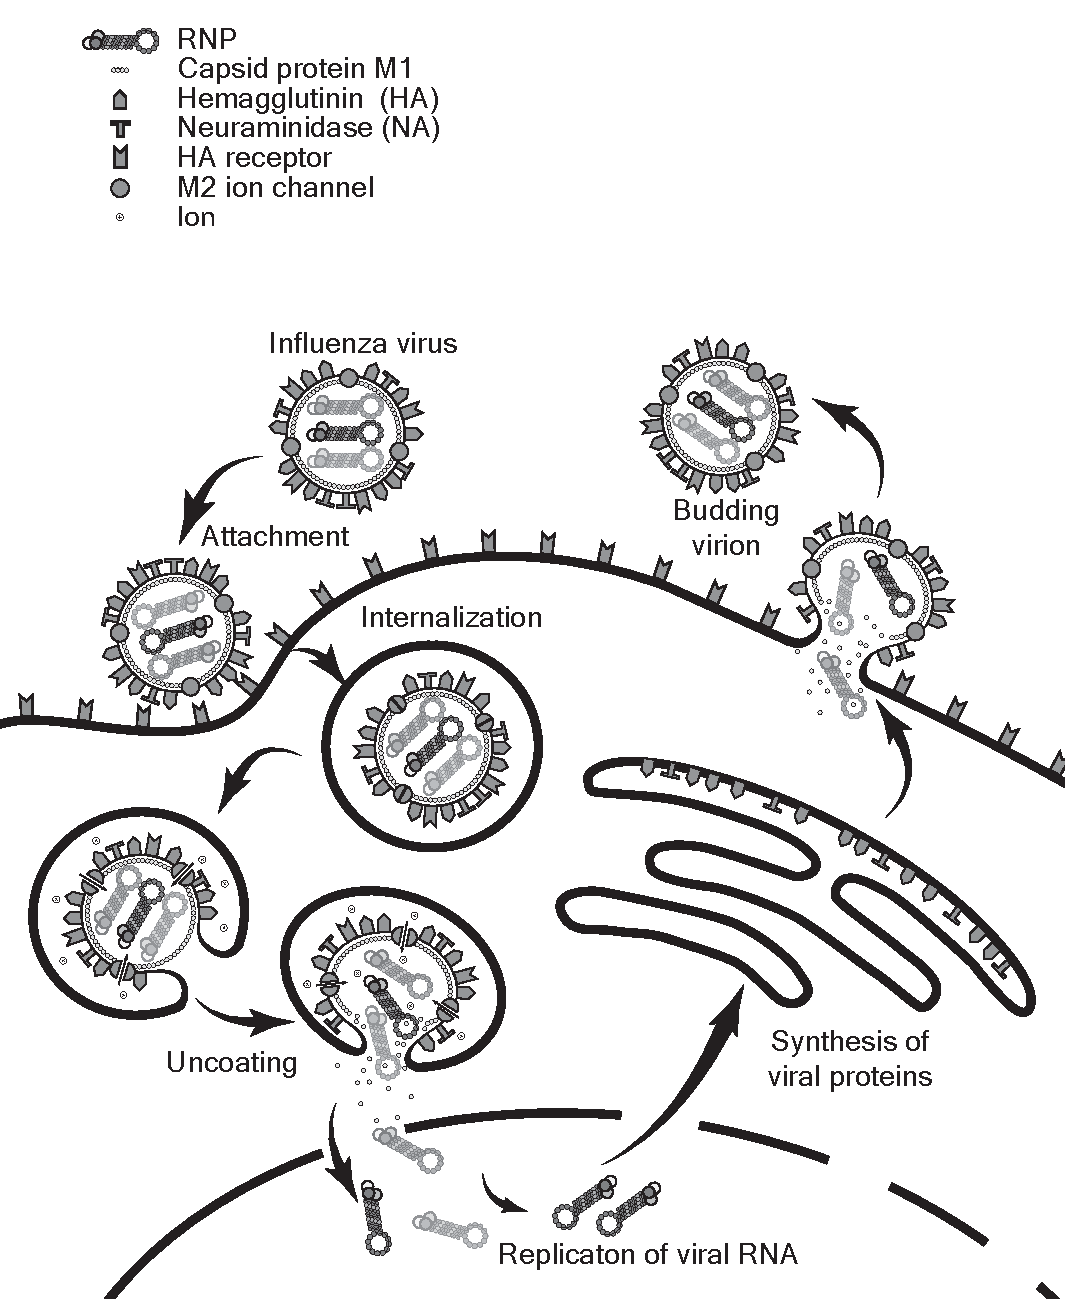
\includegraphics[width=0.95\textwidth, trim={0cm 0cm 0cm 0cm}, clip]{D_chapters/0_introduction/flu_stages.pdf}
\caption[Influenza virus infection course]{Influenza virus infection course. Refer to Figure \ref{figure:fluStructure} for details.}
\label{figure:fluInfectionStages}
\end{center}
\end{figure}

\section{Influenza Infection Prevention and Treatment}

Preventative measures, such as annual vaccination, hand washing, respiratory hygiene, and post exposure self-isolation are the best available measures in mitigating influenza infection risks \cite{influenza_seasonal_2018}.

Influenza vaccine formulation, recommended by WHO commonly includes \cite{RecommendedCompositionVaccines}

\begin{itemize}
    \item one H1N1 influenza A virus,
    \item one H3N2 influenza A virus,
    \item one or two influenza B viruses.
\end{itemize}

Influenza vaccine provides immunity to healthy adults even when formulation is not perfectly matched to circulating virus strains, but vaccination is especially important for individuals in high risk groups.

Likewise, in cases where disease occurs, for healthy adults WHO largely recommends symptomatic treatment and social distancing. For high risk groups the use of antiviral drugs is recommended \cite{influenza_seasonal_2018}.

So far, two main classes of antiviral drugs against influenza have been developed (Figure \ref{figure:fluDrugs}).

Adamantane type drugs bind to M2 ion channel, preventing endosomal acidification, which inhibits virus uncoating. In 2011 WHO reported that the majority of circulating influenza A viruses are resistant to this type of drug \cite{whoAntivirals2011}. WHO and no longer recommends adamantanes for use \cite{influenza_seasonal_2018}.

\begin{sidewaysfigure}
\begin{center}
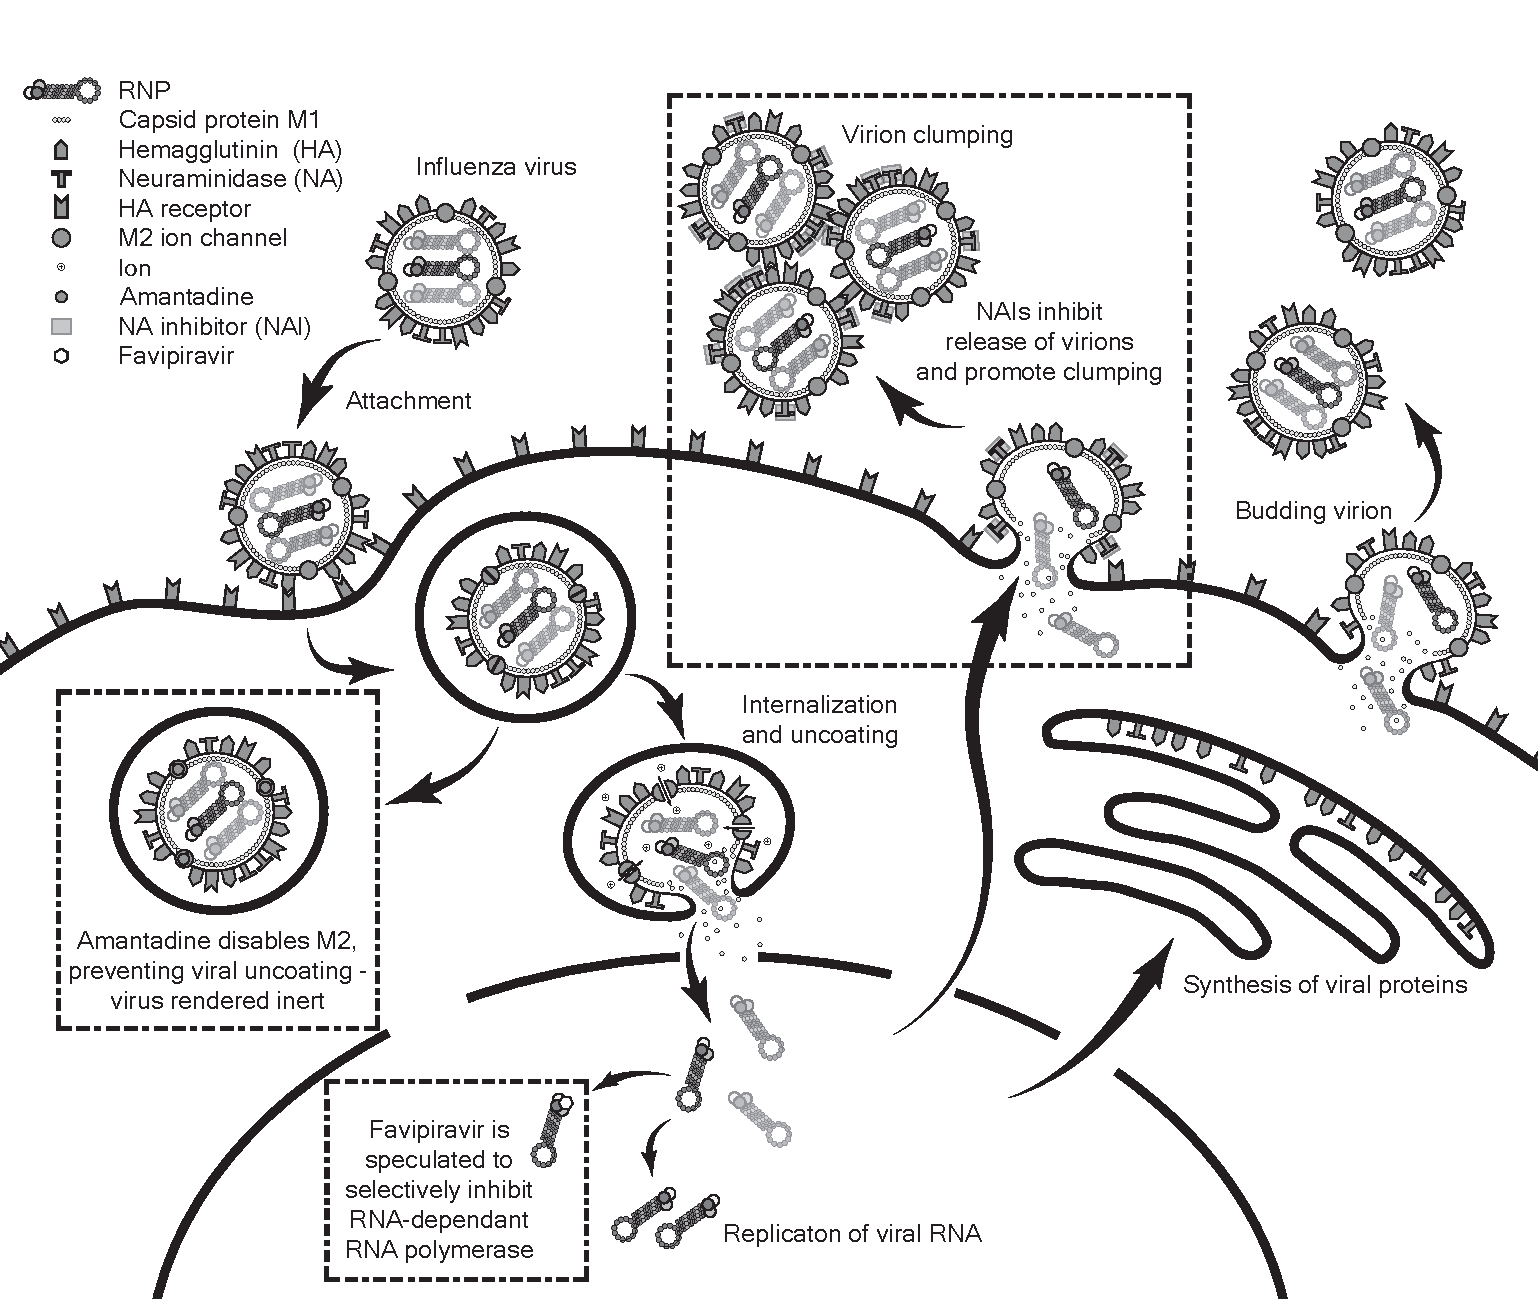
\includegraphics[width=0.75\textwidth, trim={0cm 0cm 0cm 0cm}, clip]{D_chapters/0_introduction/flu_drug.pdf}
\captionof{figure}{Mechanism of action of influenza antiviral drugs}
\label{figure:fluDrugs}
\end{center}
\end{sidewaysfigure}

Neuraminidase inhibitors bind to the viral surface enzyme neuraminidase and prevent cell surface receptor cleavage, inhibiting new virions' escape from infected cells. 2016-2017 survey reported that only about 0.2\% of collected influenza viruses showed resistance to one or more type of neuraminidase inhibitors \cite{lackenby2018global}. This type of drug remains suitable for use in the clinic, emerging resistance makes continued monitoring necessary.

Additionally, favipiravir is a broad spectrum antiviral drug, which acts as a chain terminator at the site of viral RNA incorporation \cite{shiraki2020favipiravir}. Wide applicability to a variety of viruses often comes with concerns of cellular toxicity. Favipiravir has been approved as an emergency treatment for novel (rather than seasonal) influenza viruses in Japan in 2014, however wider approval is delayed in part due to potential teratogenic concerns.


\section{Host directed anti‐viral strategies}

Currently available influenza drugs  target viral proteins M2 and NA. This approach allows for a specific mechanism of action, which, ideally, should not interfere with host cellular systems.

One significant problem with this approach is that, by introducing the antiviral drugs into the clinic, we exert evolutionary pressure on the virus. In turn, through the process of antigentic drift the virus may modify its target protein to escape inhibition by the drug, rendering the drug useless (e.g. adamantanes).

These concerns over antiviral drug resistance, and growing awareness of host proteins involvement in successful infection led to the emergence of a new drug development approach. Instead of targeting a viral protein, we try to target a host cell protein involved in viral infection. Thus, we can inhibit infection without subjecting the virus to direct selection.

\begin{figure}
\begin{center}
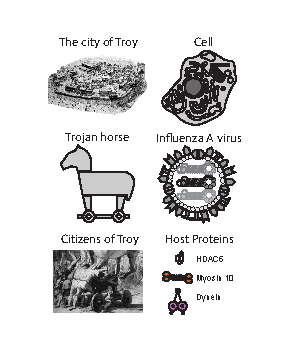
\includegraphics[width=0.7\textwidth, trim={0.6cm 0.6cm 0.6cm 0.6cm}, clip]{D_chapters/0_introduction/flu_troy.pdf}
\caption[Trojan siege metaphor for host directed anti-viral strategies]%
{Trojan siege metaphor for host directed anti-viral strategies. Refer to Figure \ref{figure:fluStructure} for details.\par The city of Troy is a black and white render of reconstruction of the Homeric city of Troy, Turkey. (Photo by DeAgostini/Getty Images). The citizens of Troy are a black and white crop of "The Procession of the Trojan Horse into Troy from Two Sketches Depicting the Trojan Horse", oil on canvas by Giovanni Domenico Tiepolo, c. 1760 in the National Gallery, London.}
\label{figure:fluTroy}
\end{center}
\end{figure}

Conceptually such an approach can be understood through the story of a Trojan siege (Figure \ref{figure:fluTroy}). Much like a Trojan horse, which could not make it inside the city without the help of its citizens, viruses require host protein help for successful infection. Choosing to target these host proteins in an antiviral treatment is alike to convincing the Trojans to leave the horse at the door.

A major challenge in host directed anti‐viral strategies is cellular toxicity (which, however, is not exclusive to this approach). It is a complex issue, which we believe is best addressed by interrogating systemically the involvement of the protein in both cellular and viral processes, as well as elucidating the specific mechanism of action of a drug-like agent.

\section{HDAC6 Structure and Function}

One such host protein with the potential to be a drug target is histone deacetylase 6 (HDAC6), along with the molecular motors myosin 10 and dynein, and their respective cytoskeletal filaments \cite{banerjee2014influenza}.

Histone deacetylases are a class of enzymes that remove acetyl groups from chromatin and other acetylated proteins. Currently 18 HDAC proteins are known, which are classified into 4 classes. HDAC6 belongs to the IIb class, which is primarily localized in the cytoplasm \cite{hai2016histone}.

Among other histone deacetylases, HDAC6 is the only one to carry tandem catalytic domains CD1 and CD2 (Figure \ref{figure:HDAC6Domains}). The dynein motor binding (DMB) domain is located between them. HDAC6 also has a ubiquitin-binding domain ZnF ("zinc-finger") which senses polyubiquitinated misfolded protein cargo \cite{hai2016histone}. HDAC6-ZnF selectively binds \cite{zhang2008mice} to ubiquitin chains with unanchored C-terminal diglycine \cite{ouyang2012protein}.

\begin{figure}
\begin{center}
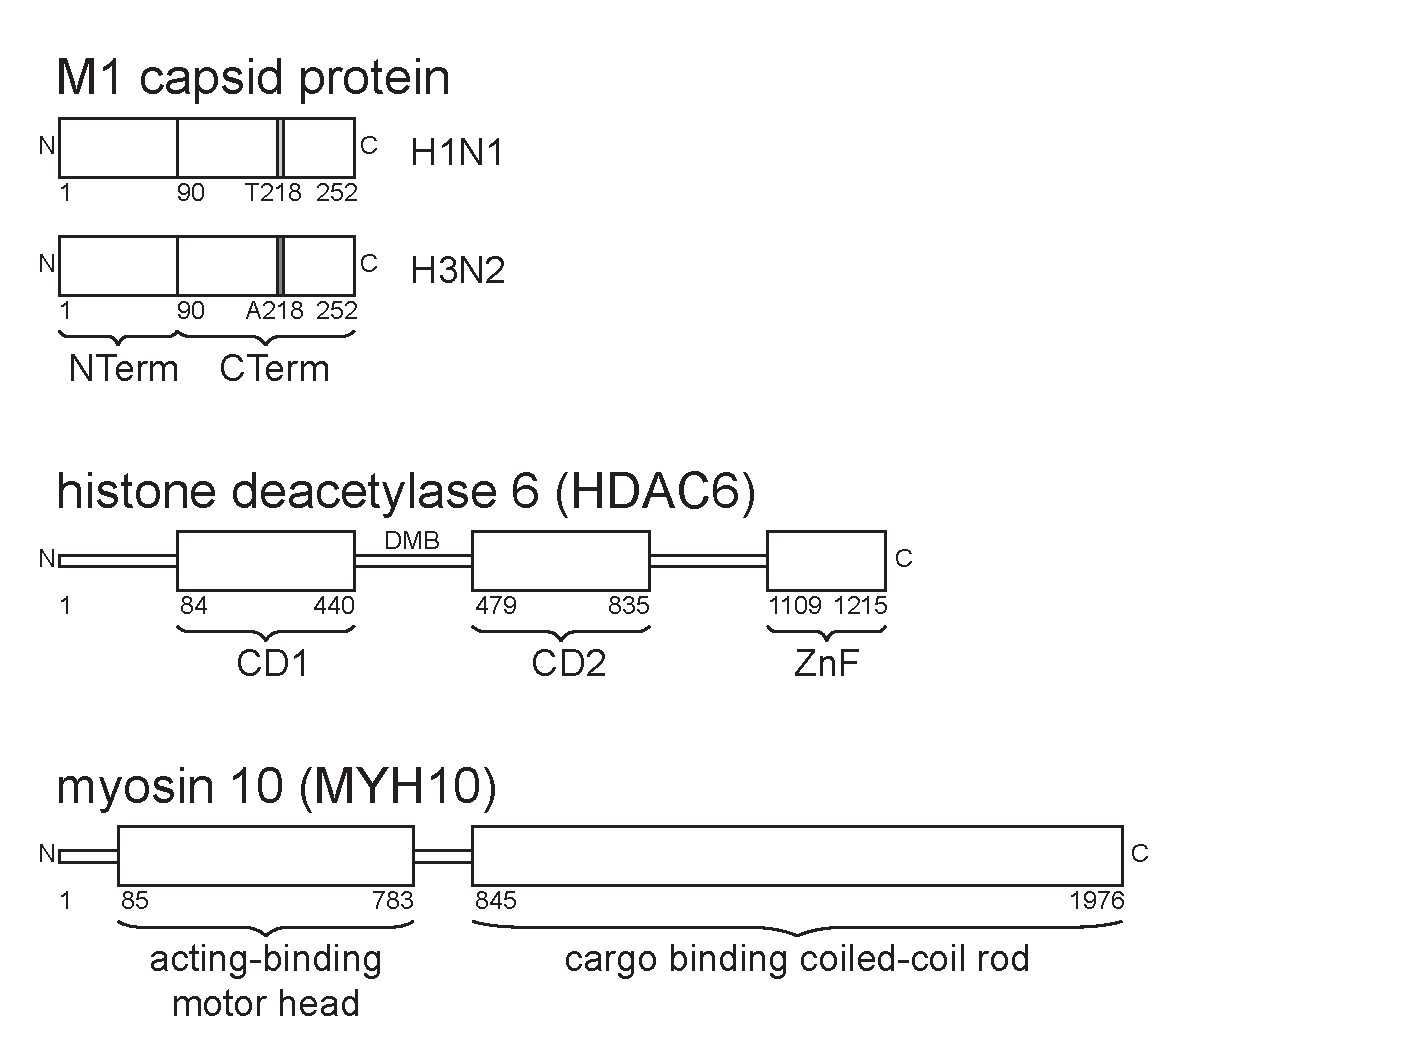
\includegraphics[width=1\textwidth, trim={0cm 6cm 8cm 8.8cm}, clip]{D_chapters/0_introduction/protein_domains.pdf}
\caption[HDAC6 domain organization]{HDAC6 domain organization \par
CD1 and CD2 - catalytic domains, DMB - dynein motor binding domain, ZnF - ubiquitin binding domain "zinc-finger". N and C denote N- and C-terminus. Numbers denote amino acid residues.}
\label{figure:HDAC6Domains}
\end{center}
\end{figure}

HDAC6 deacetylates tubulin \cite{zhang2003hdac, zhang2008mice} (polymer making up the microtubules), and heat shock protein 90 (Hsp90) \cite{kovacs2005hdac6} (a chaperone protein which assists protein folding and degradation). HDAC6 senses ubiquitinated protein aggregates and triggers their clearance \cite{boyault2007hdac6}. HCAC6 also assists in stress granule formation and cellular oxidative stress recovery \cite{kwon2007deacetylase}.

During influenza infection, HDAC6 (specifically, HDAC6-ZnF) and other components of the aggresome processing machinery - molecular motors myosin 10 and dynein - were essential for efficient uncoating. Involvement of molecular motors suggested that influenza uncoating is achieved through physical forces generated by microtubule- and actin-associated motors \cite{banerjee2014influenza}.

\section{Open questions in influenza uncoating}

Uncoating is a limiting step in influenza infection \cite{banerjee2013high}. Previously, influenza uncoating has been described as a passive process, relying on pH-controlled fusion pore formation and conformation changes in M1 capsid proteins \cite{zhang2012dissection}. Recruitment of HDAC6 and molecular motors in uncoating \cite{banerjee2014influenza} highlights that it is instead an active process which involves cellular proteins.

Molecular motors may regulate viral genome localization after uncoating \cite{qin2019real} by assisting viral transport to correct cellular compartments. This is commonly described through tug-of-war mechanism, which involves velocity and force balance between all involved parties. It has been previously suggested as a process controlling cellular cargo and viral transport \cite{gazzola2009stochastic}. Modelling studies focus on tug-of-war between two types of microtubule motors with opposing processivity \cite{muller2008tug, gazzola2009stochastic}.

Others suggest that during viral infection tug-of-war between microtubule molecular motors may act as a force generating mechanism instead \cite{strunze2011kinesin,lukic2014hiv}. Involvement of myosin 10 and dynein in both endosomal and acid bypass uncoating during influenza infection is consistent with a force generation thorugh tug-of-war between different types of molecular motors: actin filament and microtubule ones. Whether such a mechanism exist, and is able to generate enough force to break influenza capsid is unclear.

Another intriguing aspect is the role of ubiquitin (Ub) in influenza viral uncoating. Influenza virus particles carry significant amounts of cellular Ub B \cite{hutchinson2014conserved}. Ubiquitination assists viral uncoating \cite{rudnicka2016ubiquitin}. HDAC6-ZnF deletion leads to reduction of influenza uncoating \cite{banerjee2014influenza}, indicating Ub involvement in the process. One possibility is that viral Ub serves as an interface between viral capsid protein M1 and HDAC6, competing with cellular Ub. Alternatively, Ub may instead assist motor recruitment, in which case viral Ub may only provide advantage in localization, but otherwise would serve the same function as cellular Ub. These possibilities would also impact interfaces between HDAC6 and molecular motors. HDAC6 is known to bind dynein through its DMB domain \cite{kawaguchi2003deacetylase}. The exact mechanism or location of myosin interaction with HDAC6 is unclear.
